\documentclass[conference]{IEEEtran}
\usepackage[pdftex]{graphicx}
\usepackage{cite}

% correct bad hyphenation here
\hyphenation{op-tical net-works semi-conduc-tor}

\begin{document}
%
% paper title
% can use linebreaks \\ within to get better formatting as desired
% Do not put math or special symbols in the title.
\title{Multiagent Coordination in Roombas: From a Neural Network Perspective}


% author names and affiliations
% use a multiple column layout for up to three different
% affiliations
\author{\textbf{Jimmy Xin Lin} and \textbf{Barry Feigenbaum}}

% use for special paper notices
%\IEEEspecialpapernotice{(Invited Paper)}

% make the title area
\maketitle

% As a general rule, do not put math, special symbols or citations
% in the abstract
\begin{abstract}
The abstract goes here.
\end{abstract}

\IEEEpeerreviewmaketitle



\section{Introduction}
Most of existing literatures about Roomba is qualitative.

\section{Related Works}
\subsection{Coordinated Multiagent Reinforcement Learning}
\cite{nguyen2014decentralized} Existing work typically assumes that the prob- lem in each time step is decoupled from the problems in other time steps, which might not hold in some applications. Therefore, in this paper, we make the following contributions: (i) We introduce a new model, called Markovian Dynamic DCOPs (MD-DCOPs), where the DCOP in the next time step is a function of the value assignments in the current time step; (ii) We introduce two distributed reinforcement learning algo- rithms, the Distributed RVI Q-learning algorithm and the Dis- tributed R-learning algorithm, that balance exploration and exploitation to solve MD-DCOPs in an online manner; and (iii) We empirically evaluate them against an existing multi- arm bandit DCOP algorithm on dynamic DCOPs.

\cite{zhang2011coordinated} This paper presents a
model-free, scalable learning approach that synthesizes
multi-agent reinforcement learning (MARL) and distributed
constraint optimization (DCOP). By exploiting
structured interaction in ND-POMDPs, our approach
distributes the learning of the joint policy and employs
DCOP techniques to coordinate distributed learning to
ensure the global learning performance. Our approach
can learn a globally optimal policy for ND-POMDPs
with a property called groupwise observability. Experimental
results show that, with communication during
learning and execution, our approach significantly outperforms
the nearly-optimal non-communication policies
computed offline.

SBDO: A New Robust Approach to Dynamic Distributed Constraint Optimisation

\cite{zhang2013coordinating}

\cite{banerjee2012sample}

\cite{kraemer2012informed}

\cite{}
Complex problems involving multiple agents exhibit varying degrees of
cooperation. The levels of cooperation might reflect both differences in
information as well as differences in goals. In this research, we develop a
general mathematical model for distributed, semi-cooperative planning and
suggest a solution strategy which involves decomposing the system into
subproblems, each of which is specified at a certain period in time and
controlled by an agent. The agents communicate marginal values of resources to
each other, possibly with distortion. We design experiments to demonstrate the
benefits of communication between the agents and show that, with
communication, the solution quality approaches that of the ideal situation
where the entire problem is controlled by a single agent.

\cite{sen1994learning}
Researchers in the field of Distributed Artificial
Intelligence (DAI) have been developing efficient
mechanisms to coordinate the activities of multiple
autonomous agents. The need for coordination
arises because agents have to share resources
and expertise required to achieve their goals.
Previous work in the area includes using sophisticated
information exchange protocols, investigating
heuristics for negotiation, and developing
formal models of possibilities of conflict and cooperation
among agent interests. In order to handle
the changing requirements of continuous and
dynamic environments, we propose learning as a
means to provide additional possibilities for effective
coordination. We use reinforcement learning
techniques on a block pushing problem to show
that agents can learn complimentary policies to
follow a desired path without any knowledge
about each other. We theoretically analyze and
experimentally verify the effects of learning rate
on system convergence, and demonstrate benefits
of using learned coordination knowledge on similar
problems. Reinforcement learning based coordination
can be achieved in both cooperative and
non-cooperative domains, and in domains with
noisy communication channels and other stochastic
characteristics that present a formidable c
\subsection{Coordinated Multiagent Neuroevolution}

\section{Problem Formulation}

\subsection{Structure of Roomba Environment}
The Roomba environment, under the OpenNERO platform \cite{karpov2008opennero},
is a virtual computer lab with crumbs distributed on the floor.
In this virtual lab, there are four classes of objects: agents, crumbs, walls,
decorations. 
Vacuum cleaner agents (grey cylinders) are supposed to collect the static
crumbs (blue cubes).  
The agents will be rewarded if they move to a place covering any crumb. 
Walls are also set up as the limits of the Roomba environment, such that
agents are not allowed to move beyond the walls and no pellets can be put
outside the walls.
Other decorative objects within the computer lab include tables, chairs, and
computers. For simplicity at the moment, these decorations only serve as
physically transparent decorations, which means they do not block agents' movements.

In the Roombas environment, the movements of vacuum cleaner agents are not
constrained by four directions (left, right, forward, backward). Instead,
agents are able to move towards all directions and each moving action is
denoted as a continuous radius value.

Three different modes (MANUAL, RANDOM, and CLUSTER) are employed to specify
the placing position of each individual crumb.
In the MANUAL mode,
one pellet is deterministically placed at a user-specified position. In the
RANDOM mode, the placement of one pellet is totally randomized; the
environment will throw a rejection and repeat the random generation, if an
invalid position is yielded. The last one is the CLUSTER mode, where the
environment samples the position of one pellet from a gaussian distribution
whose centers and spreads at $x$ and $y$ coordinates are specified. 
% in our experiment
It goes without any doubt that 

Sensors of Agents. Initial sensors.

Rewards/penalty design.



\begin{figure}[!t]
\centering
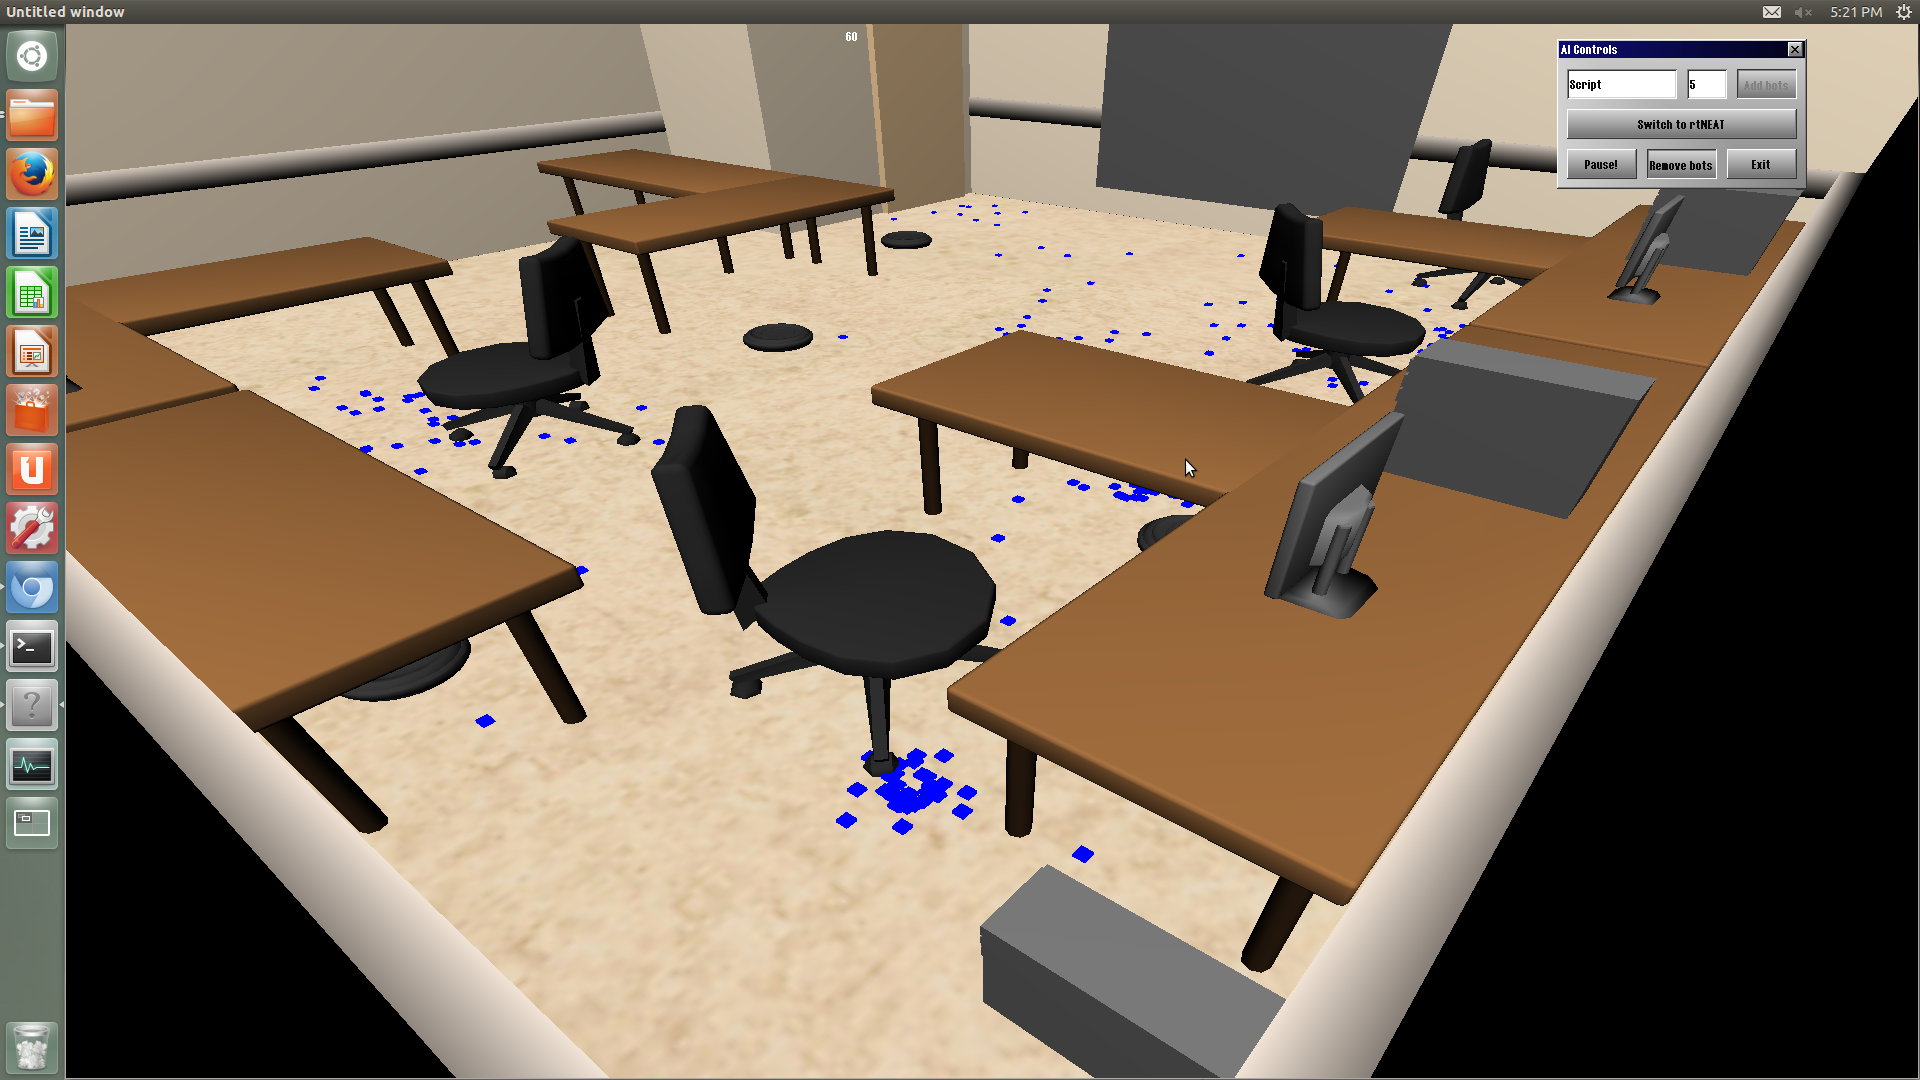
\includegraphics[width=3.2in,height=2.1in]{./figures/roombas/roomba2.png}
\caption{Overall Picture of the Roomba Environment}
\label{fig_sim}
\end{figure}


\subsection{Multiagent Behaviors}

\subsection{Difficulties and Challenges}

\section{Experiments: Initial Setup}
This section will present some preliminary results coming from the simulation
of greedy agents. Agents with greedy strategy simply approaches to the direction
where the closest pellet to it is there.  These results may not be directly
related to the multiagent behaviors, but 
(i) demonstrate that we have set up the environment correctly from both
reinforcement learning and neuroevolution. 
(ii) illustrate intuitively the benchmark intelligence for the crumb
collection.

\subsection{Reinforcement Learning}
Add implementation details of Q-Learning and variants here...

\subsection{Neuroevolution}
Add implementation details of Neuroevolution here...

\section{Experiments: Multiagent Coordination}

%\begin{figure}[!t]
%\centering
%\includegraphics[width=2.5in]{myfigure}
%\caption{Simulation Results.}
%\label{fig_sim}
%\end{figure}



\section{Conclusions}
The conclusion goes here. 

Future Works go here.

% trigger a \newpage just before the given reference
% number - used to balance the columns on the last page
% adjust value as needed - may need to be readjusted if
% the document is modified later
%\IEEEtriggeratref{8}
% The "triggered" command can be changed if desired:
%\IEEEtriggercmd{\enlargethispage{-5in}}

% references section

% can use a bibliography generated by BibTeX as a .bbl file
% BibTeX documentation can be easily obtained at:
% http://www.ctan.org/tex-archive/biblio/bibtex/contrib/doc/
% The IEEEtran BibTeX style support page is at:
% http://www.michaelshell.org/tex/ieeetran/bibtex/

\bibliographystyle{IEEEtran}
\bibliography{report}

% <OR> manually copy in the resultant .bbl file
% set second argument of \begin to the number of references
% (used to reserve space for the reference number labels box)

%\begin{thebibliography}{1}
%\bibitem{IEEEhowto:kopka}
%H.~Kopka and P.~W. Daly, \emph{A Guide to \LaTeX}, 3rd~ed.\hskip 1em plus
%  0.5em minus 0.4em\relax Harlow, England: Addison-Wesley, 1999.
%\end{thebibliography}




% that's all folks
\end{document}
